\documentclass[crop,tikz]{standalone}
\usepackage{tkz-euclide}
\usetikzlibrary{arrows.meta}
\usetkzobj{all}
\usetikzlibrary{shapes}


\tikzstyle{myarrows}=[line width=1mm,draw=blue,-triangle 45,postaction={draw, line width=3mm, shorten >=4mm, -}]
\begin{document}

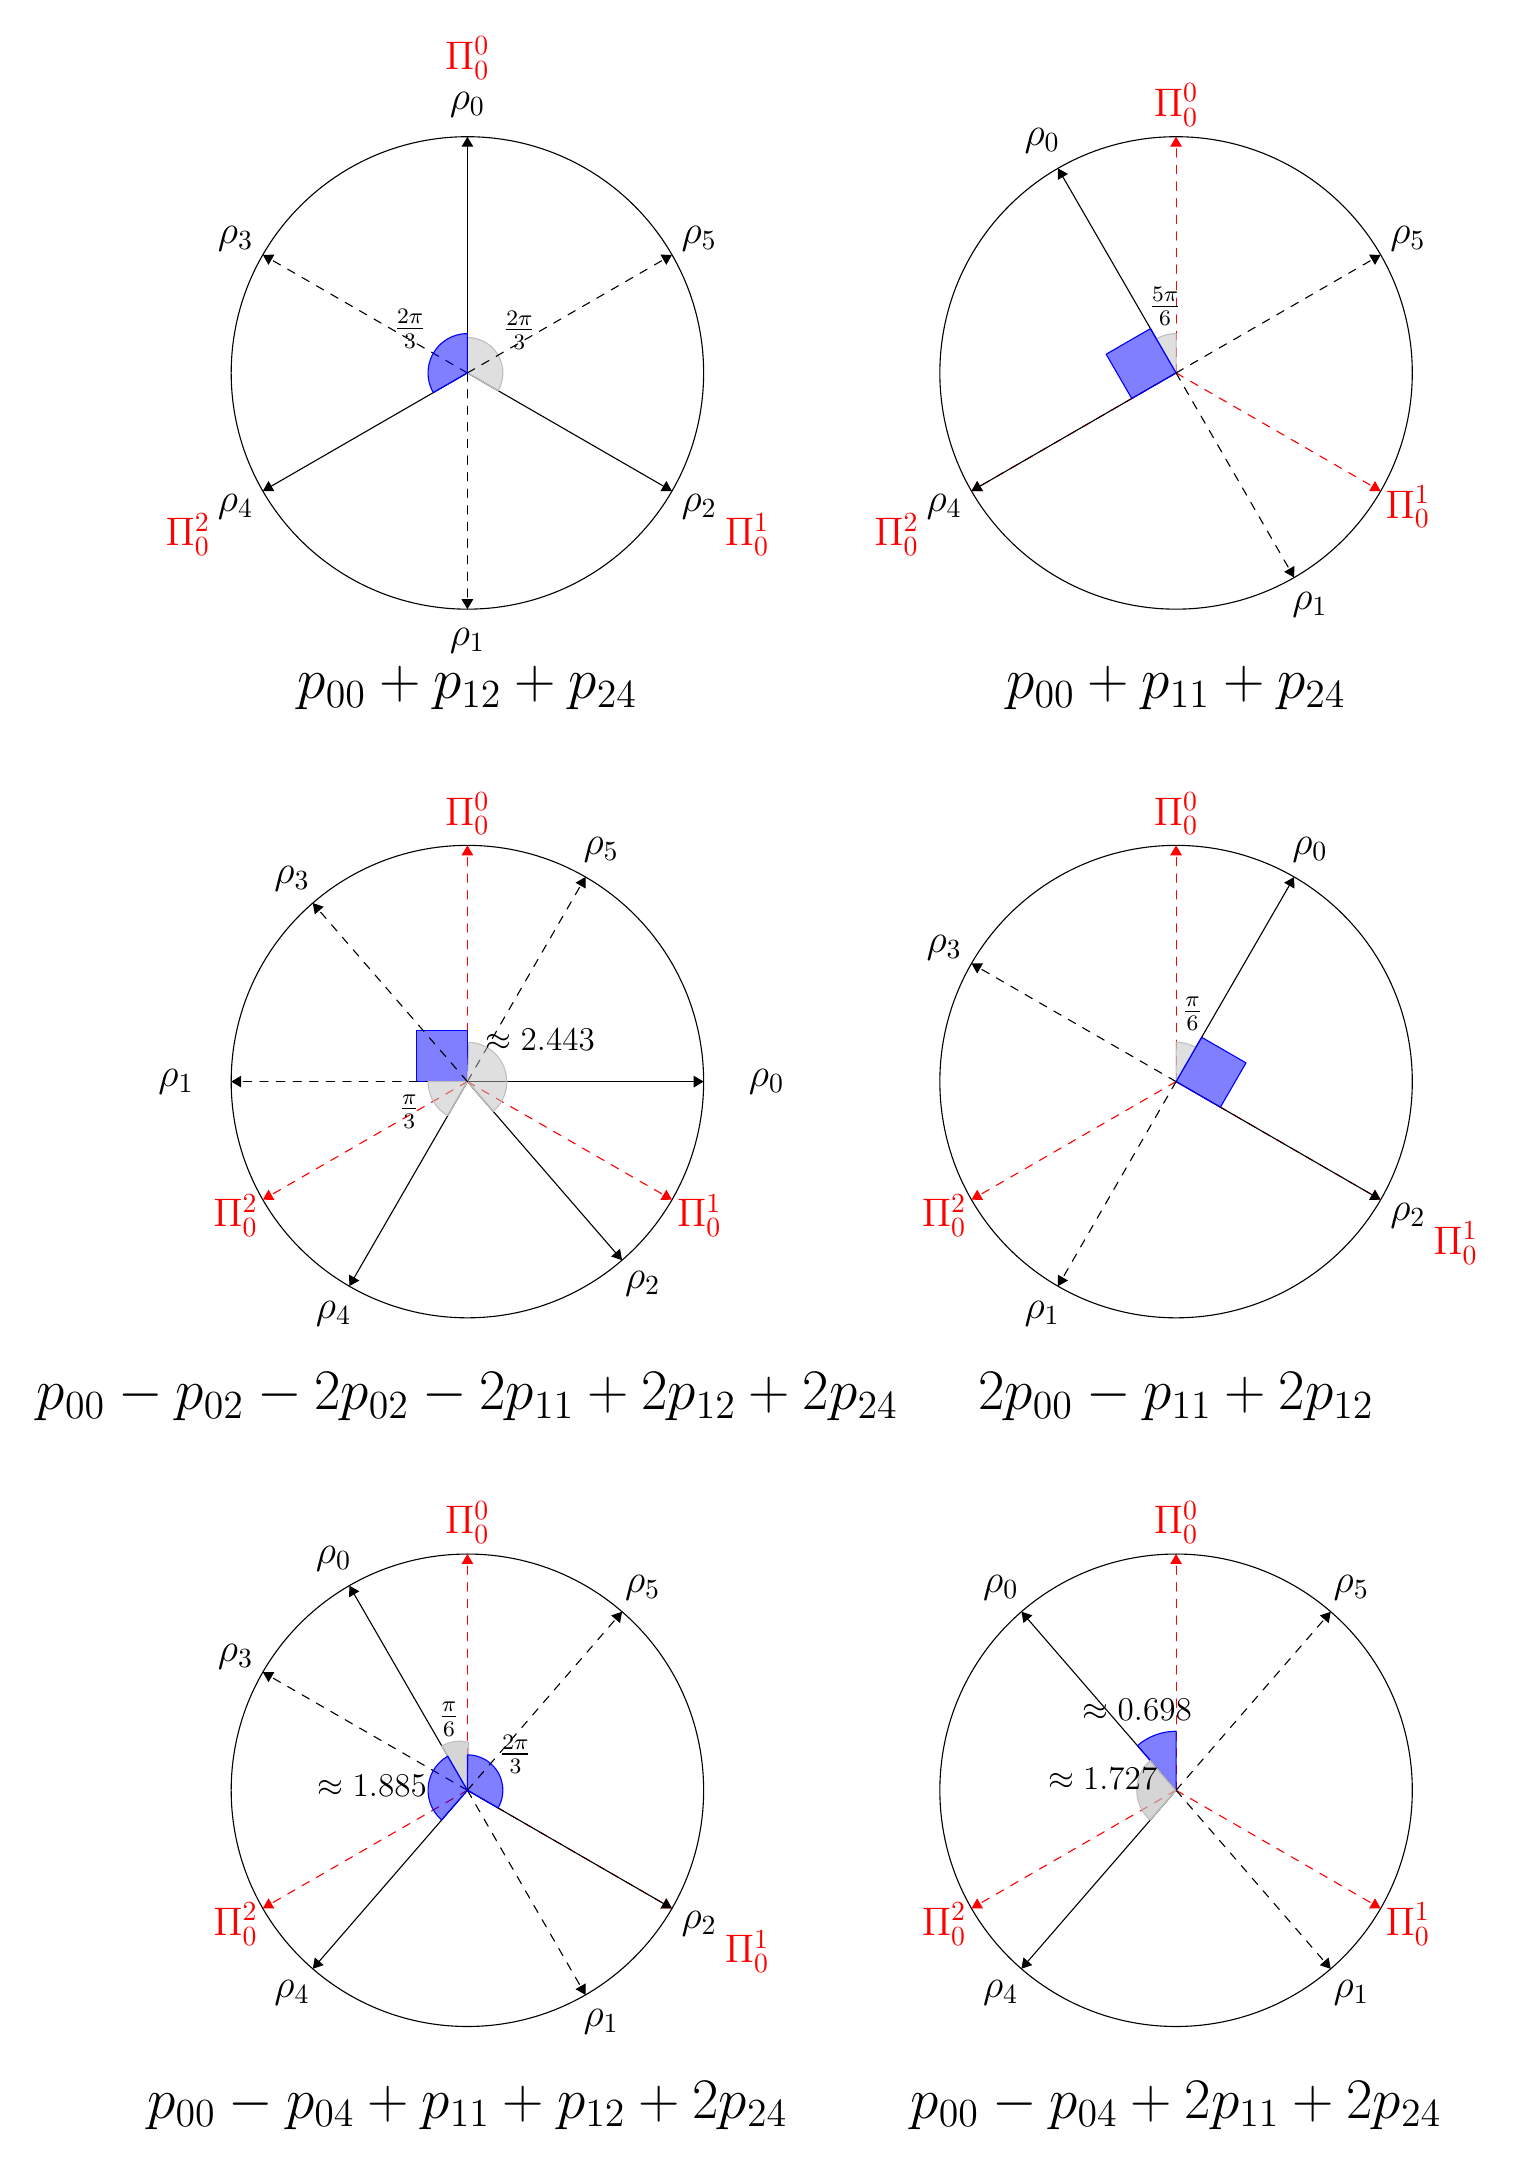
\begin{tikzpicture}[line cap=round, line join=round, >=Triangle]

%\node at (-4.5,5) {\Huge $\{\rho_x\}^5_{x=0}$,{\color{red} $\{\Pi^y_0\}^2_{y=0}$} };
\begin{scope}[ shift={(-9,0)}]
\draw  (0,0) ellipse (3 and 3);


\draw[->]  (0,0) -- (0,3);
\draw (0,3.4) node {\Large $\rho_0$};
	\draw (0,4.) node {\Large \color{red} $\Pi_0^0$};

\draw[->,dashed]  (0,0)  -- (0,-3);
\draw (0,-3.4) node {\Large $\rho_1$};



\begin{scope}[rotate=-120]    
	\draw[->]  (0,0)  -- (0,3);
	\draw (0,3.4) node {\Large $\rho_2$};
	\draw (0,4.1) node {\color{red}  \Large \color{red}  $\Pi_0^1$};
	\draw[->,dashed]  (0,0)  -- (0,-3);
	\draw (0,-3.4) node {\Large $\rho_3$};
	\draw [lightgray, fill, fill opacity=0.5]  (0,0) -- (90:0.45) arc (90:210:0.45) -- cycle;
	\node at (-0.8,0.3) {\large $\frac{2\pi}{3}$};
\end{scope}



\begin{scope}[rotate=120]    
	\draw[->]  (0,0)  -- (0,3);
	\draw (0,3.4) node {\Large $\rho_4$};
	\draw (0,4.1) node {\color{red}  \Large $\Pi_0^2$};
	\draw[->,dashed]  (0,0)  -- (0,-3);
	\draw (0,-3.4) node {\Large $\rho_5$};
	\draw [shift={(0,0)}, blue, fill, fill opacity=0.5] (0,0) -- (90:0.5) arc (90:-30:0.5) -- cycle;
\node at (0.85,0.35) {\large $\frac{2\pi}{3}$};
\end{scope}


\node at (0,-4) {\huge $p_{00} +p_{12} +p_{24} $};
\end{scope}

%---------------------------------------------------------------------------------------------------
%\begin{scope}[ shift={(8,0)}]
%\draw  (0,0) ellipse (3 and 3);


%\draw[->]  (0,0) -- (0,3);
%\draw (0,3.4) node {\Large $\Pi^0_0$};




%\begin{scope}[rotate=-120]    
%	\draw[->]  (0,0)  -- (0,3);
%	\draw (0,3.4) node {\Large $\Pi^1_0$};
%	\draw [lightgray, fill, fill opacity=0.5]  (0,0) -- (90:0.45) arc (90:210:0.45) -- cycle;
%	\node at (-0.8,0.3) {\large $\frac{2\pi}{3}$};
%\end{scope}




%\begin{scope}[rotate=120]    
%	\draw[->]  (0,0)  -- (0,3);
%\draw (0,3.4) node {\Large $\Pi^2_0$};
%\draw [shift={(0,0)}, blue, fill, fill opacity=0.5] (0,0) -- (90:0.5) arc (90:-30:0.5) -- cycle;
%\node at (0.85,0.35) {\large $\frac{2\pi}{3}$};
%\end{scope}



%\node at (0,4.5) {\huge $\{\Pi^y_k\}$ };
%\end{scope}

%---------------------------------------------------------------------------------------------------












%---------------------------------------------------------------------------------------------------

\begin{scope}[ shift={(0,0)}]
\draw  (0,0) ellipse (3 and 3);
\draw (0,3.4) node {\Large \color{red} $\Pi^0_0$};
\draw[->,dashed,red]  (0,0) -- (0,3);
\begin{scope}[rotate=-120]  
\draw[->,dashed,red]  (0,0) -- (0,3);
\draw (0,3.4) node {\Large \color{red} $\Pi^1_0$};
\end{scope}
\begin{scope}[rotate=120]  
\draw[->,dashed,red]  (0,0) -- (0,3);
\draw (0,4.1) node {\Large \color{red} $\Pi^2_0$};
\end{scope}

\begin{scope}[ rotate =30]
\draw[->]  (0,0) -- (0,3);
\draw (0,3.4) node {\Large $\rho_0$};
\draw[->,dashed]  (0,0)  -- (0,-3);
	\draw (0,-3.4) node {\Large $\rho_1$};
\draw [shift={(0,0)},lightgray, fill, fill opacity=0.5] (0,0) -- (90:0.5) arc (90:60:0.5) -- cycle;
\node at (0.3,0.8) {\large $\frac{5\pi}{6}$};

\begin{scope}[rotate=90]    
	\draw[->]  (0,0)  -- (0,3);
	\draw (0,3.4) node {\Large $\rho_4$};
\draw [shift={(0,0)}, blue, fill, fill opacity=0.5] (0,0) rectangle (0.65,0.65);
\draw[->,dashed]  (0,0)  -- (0,-3);
	\draw (0,-3.4) node {\Large $\rho_5$};
\end{scope}

\end{scope}
\node at (0,-4) {\huge $p_{00} +p_{11} +p_{24}$ };
\end{scope}
%---------------------------------------------------------------------------------------------------












\begin{scope}[ shift={(-9,-9)}]
\draw  (0,0) ellipse (3 and 3);

\draw[->,dashed,red]  (0,0) -- (0,3);
\draw (0,3.4) node {\Large \color{red} $\Pi^0_0$};
\begin{scope}[rotate=-120]  
\draw[->,dashed,red]  (0,0) -- (0,3);
\draw (0,3.4) node {\Large \color{red} $\Pi^1_0$};
\end{scope}
\begin{scope}[rotate=120]  
\draw[->,dashed,red]  (0,0) -- (0,3);
\draw (0,3.4) node {\Large \color{red} $\Pi^2_0$ };
\end{scope}

\begin{scope}[ rotate =-90]
\draw[->]  (0,0) -- (0,3);
\draw (0,3.8) node {\Large $\rho_0$};
\draw [shift={(0,0)}, blue, fill, fill opacity=0.5] (0,0) rectangle (-0.65,-0.65);
\draw[->,dashed]  (0,0)  -- (0,-3);
	\draw (0,-3.7) node {\Large $\rho_1$};





\begin{scope}[rotate=-120]    
	\draw[->]  (0,0)  -- (0,3);
	\draw (0,3.4) node {\Large $\rho_4$};
	\draw [shift={(0,0)}, lightgray, fill, fill opacity=0.5] (0,0) -- (90:0.5) arc (90:30:0.5) -- cycle;
\node at (	0.45,0.7) {\large $\frac{\pi}{3}$};
\draw[->,dashed]  (0,0)  -- (0,-3);
	\draw (0,-3.4) node {\Large $\rho_5$};
\end{scope}



\end{scope}

\begin{scope}[rotate=-139.1]    
	\draw[->]  (0,0)  -- (0,3);
	\draw (0,3.4) node {\Large $\rho_2$};
	\draw [shift={(0,0)}, lightgray, fill, fill opacity=0.5] (0,0) -- (90:0.5) arc (90:180+46.9:0.5) -- cycle;
\node at (-1.05,0.2) {\large $\approx 2.443$};
\draw[->,dashed]  (0,0)  -- (0,-3);
	\draw (0,-3.4) node {\Large $\rho_3$};
\end{scope}
\node at (0,-4) {\huge $p_{00} -p_{02} - 2 p_{02}-2 p_{11} +2 p_{12} +2 p_{24}$ };

\end{scope}



%---------------------------------------------------------------------------------------------------









\begin{scope}[ shift={(0,-9)}]
\draw  (0,0) ellipse (3 and 3);


\draw[->,dashed,red]  (0,0) -- (0,3);
\draw (0,3.4) node {\Large \color{red} $\Pi^0_0$};
\begin{scope}[rotate=-120]  
\draw[->,dashed,red]  (0,0) -- (0,3);
\draw (0,4.1) node {\Large \color{red} $\Pi^1_0$};
\end{scope}
\begin{scope}[rotate=120]  
\draw[->,dashed,red]  (0,0) -- (0,3);
\draw (0,3.4) node {\Large \color{red} $\Pi^2 _0$};
\end{scope}

\begin{scope}[ rotate =-30]

\draw[->]  (0,0) -- (0,3);
\draw (0,3.4) node {\Large $\rho_0$};
\draw [shift={(0,0)}, lightgray, fill, fill opacity=0.5] (0,0) -- (90:0.5) arc (90:120:0.5) -- cycle;
\node at (-0.25,0.85) {\large $\frac{\pi}{6}$};
\draw[->,dashed]  (0,0)  -- (0,-3);
	\draw (0,-3.4) node {\Large $\rho_1$};
\begin{scope}[rotate=-90]    
	\draw[->]  (0,0)  -- (0,3);
	\draw (0,3.4) node {\Large $\rho_2$};
	\draw [shift={(0,0)},blue, fill, fill opacity=0.5] (0,0) rectangle (-0.65,0.65);
	\draw[->,dashed]  (0,0)  -- (0,-3);
	\draw (0,-3.4) node {\Large $\rho_3$};
\end{scope}


%---------------------------------------------------------------------------------------------------
\end{scope}
\node at (0,-4) {\huge $2p_{00} - p_{11} + 2 p_{12}$ };

\end{scope}










%---------------------------------------------------------------------------------------------------
\begin{scope}[ shift={(-9,-18)}]
\draw  (0,0) ellipse (3 and 3);
\draw (0,3.4) node {\Large \color{red} $\Pi^0_0$};
\draw[->,dashed,red]  (0,0) -- (0,3);
\begin{scope}[rotate=-120]  
\draw[->,dashed,red]  (0,0) -- (0,3);
\draw (0,4.1) node {\Large \color{red} $\Pi^1_0$};
\end{scope}
\begin{scope}[rotate=120]  
\draw[->,dashed,red]  (0,0) -- (0,3);
\draw (0,3.4) node {\Large \color{red} $\Pi^2_0$};
\end{scope}

\begin{scope}[ rotate =30]

\draw[->]  (0,0) -- (0,3);
\draw (0,3.4) node {\Large $\rho_0$};
	\draw [ lightgray, fill, fill opacity=0.65]  (0,0) -- (90:0.65) arc (90:45:0.45) -- cycle;
\node at (0.25,0.9) {\large $\frac{\pi}{6}$};
\draw[->,dashed]  (0,0)  -- (0,-3);
	\draw (0,-3.4) node {\Large $\rho_1$};


\begin{scope}[rotate=-150]    
	\draw[->]  (0,0)  -- (0,3);
	\draw (0,3.4) node {\Large $\rho_2$};
	\draw [ blue, fill, fill opacity=0.5]  (0,0) -- (90:0.45) arc (90:210:0.45) -- cycle;
	\node at (-0.7,0.3) {\large $\frac{2\pi}{3}$};
	\draw[->,dashed]  (0,0)  -- (0,-3);
	\draw (0,-3.4) node {\Large $\rho_3$};
\end{scope}




\begin{scope}[rotate=109.1]    
	\draw[->]  (0,0)  -- (0,3);
	\draw (0,3.4) node {\Large $\rho_4$};
	\draw [shift={(0,0)}, blue, fill, fill opacity=0.5] (0,0) -- (90:0.5) arc (90:-30+10.9:0.5) -- cycle;
\node at (0.95,0.75) {\large $\approx1.885$};
\draw[->,dashed]  (0,0)  -- (0,-3);
	\draw (0,-3.4) node {\Large $\rho_5$};
\end{scope}


\end{scope}
\node at (0,-4) {\huge $p_{00}  - p_{04} +   p_{11} + p_{12} +2 p_{24}$ };

\end{scope}

%---------------------------------------------------------------------------------------------------












%---------------------------------------------------------------------------------------------------
\begin{scope}[ shift={(0,-18)}]
\draw  (0,0) ellipse (3 and 3);
\draw (0,3.4) node {\Large \color{red} $\Pi^0_0$};


\draw[->,dashed,red]  (0,0) -- (0,3);
\begin{scope}[rotate=-120]  
\draw (0,3.4) node {\Large \color{red} $\Pi^1_0$};
\draw[->,dashed,red]  (0,0) -- (0,3);
\end{scope}
\begin{scope}[rotate=120]  
\draw (0,3.4) node {\Large \color{red} $\Pi^2_0$};
\draw[->,dashed,red]  (0,0) -- (0,3);
\end{scope}

\begin{scope}[ rotate =40.89]

\draw[->]  (0,0) -- (0,3);
\draw (0,3.4) node {\Large $\rho_0$};
	\draw [shift={(0,0)}, blue, fill, fill opacity=0.5] (0,0) -- (90:0.75) arc (90:90-40.89:0.75) -- cycle;
\node at (0.3,1.1 ) {\large $\approx0.698$};
\draw[->,dashed]  (0,0)  -- (0,-3);
	\draw (0,-3.4) node {\Large $\rho_1$};

\begin{scope}[rotate=98.2]    
	\draw[->]  (0,0)  -- (0,3);
	\draw (0,3.4) node {\Large $\rho_4$};
	\draw [shift={(0,0)},lightgray, fill, fill opacity=0.65] (0,0) -- (90:0.5) arc (90:-30+21.8:0.5) -- cycle;
\node at (0.8,0.5) {\large $\approx1.727$};
\draw[->,dashed]  (0,0)  -- (0,-3);
	\draw (0,-3.4) node {\Large $\rho_5$};
\end{scope}


\end{scope}
\node at (0,-4) {\huge $p_{00}  - p_{04} +   2p_{11}  +2 p_{24}$ };

\end{scope}

%---------------------------------------------------------------------------------------------------


\end{tikzpicture}

\end{document}